\documentclass{article}
\usepackage[utf8]{inputenc}
\usepackage{fontspec}
\usepackage{textcomp}
\usepackage{graphicx}
\usepackage{hyperref}
\usepackage{caption}
\usepackage{float}
\usepackage{amsmath, amssymb, amsfonts}
\usepackage{xcolor}
\usepackage{geometry}
\usepackage{enumitem}
\usepackage{titlesec}
\usepackage[backend=biber, style=numeric]{biblatex} 
\addbibresource{bibliography.bib} 

\geometry{a4paper, margin=1in}

\setmainfont{Latin Modern Roman}

\titlespacing*{\section}{0pt}{12pt plus 4pt minus 2pt}{6pt plus 2pt minus 2pt}
\titlespacing*{\subsection}{0pt}{10pt plus 3pt minus 2pt}{4pt plus 2pt minus 2pt}

\setlist[itemize]{leftmargin=*, itemsep=2pt, parsep=0pt, topsep=4pt}

\newcommand{\firstauthorname}{Julian Bednarek}
\newcommand{\secondauthorname}{Hubert Szadkowski}
\newcommand{\thirdauthorname}{Bartłomiej Sęczkowski}
\newcommand{\fourthauthorname}{Jakub Raj}
\newcommand{\fifthauthorname}{Diana Prośniewska}
\newcommand{\universityname}{Lodz University of Technology, Poland}
\newcommand{\supervisorname}{Bartosz Sakowicz}
\newcommand{\supervisoremail}{bartosz.sakowicz@p.lodz.pl}
\newcommand{\projecttitle}{Table Hub Mobile App for Restaurant Table Management}
\newcommand{\teamname}{Team 5}
\newcommand{\coursename}{CS}

\hypersetup{
    colorlinks=true,
    linkcolor=blue,
    filecolor=magenta,
    urlcolor=cyan,
}

\usepackage{url}
\usepackage{ragged2e}
\raggedbottom 

\renewcommand{\textfraction}{0.05}
\renewcommand{\topfraction}{0.95}
\renewcommand{\bottomfraction}{0.95}
\setcounter{totalnumber}{5}
\setcounter{topnumber}{5}
\setcounter{bottomnumber}{5}


\begin{document}

\title{\projecttitle}
\author{
    \firstauthorname\textsuperscript{1}\\
    \secondauthorname\textsuperscript{1}\\
    \thirdauthorname\textsuperscript{1}\\
    \fourthauthorname\textsuperscript{1}\\
    \fifthauthorname\textsuperscript{1}\\[1ex]
    \textsuperscript{1}\universityname\\[1ex]
    Supervisor: \supervisorname{} (e-mail: \supervisoremail)
}
\date{June 2025}

\maketitle

\begin{abstract}
This report presents the Table Hub Mobile application, designed to revolutionize restaurant table management. Traditional methods often lead to inefficiencies, inaccurate information, and frustrated customers, particularly due to spontaneous outings and difficulties finding free tables during peak hours. The Table Hub application directly addresses these pain points by providing accurate, real-time table status updates through an intuitive user-friendly interface for both restaurant staff and customers. Key functionalities include an interactive floor plan and real-time WebSocket communication to ensure data consistency across all users. Developed for Android using Kotlin and Jetpack Compose, the application leverages modern development practices such as MVVM architecture and Hilt for dependency injection, ensuring maintainability and scalability. The solution aims to enhance the dining experience, reduce frustration, and streamline restaurant operations.
\end{abstract}

\noindent\textbf{KEYWORDS:} Android, Kotlin, Jetpack Compose, WebSocket, Table Management, Restaurant, Mobile Application, Hilt

\section{Introduction}
This document outlines the final report for the Table Hub Mobile application project. Our team aims to streamline the process of managing restaurant table availability, providing a user-friendly interface for both restaurant staff and customers to quickly ascertain and update table statuses.

\subsection{Background Information}
The traditional method of tracking restaurant table availability often relies on manual observation or rudimentary systems, leading to inefficiencies, inaccurate information, and potential loss of revenue due to mismanaged seating. Customers frequently face uncertainty regarding table availability, and staff can be overwhelmed during peak hours trying to coordinate seating. This problem scales with the size and popularity of the restaurant, as well as the complexity of its layout with multiple sections.

\subsection{Problem Finding}
Our detailed user research, including a survey, highlighted several key pain points in restaurant table management. The survey revealed that \textbf{over 74\% of respondents (specifically 78\% combining "often" and "very often" responses) indicated that their outings are spontaneous}, rather than pre-planned. This spontaneity frequently leads to difficulties, as approximately \textbf{74\% of respondents reported problems finding a free table during peak hours}, a situation particularly prevalent on busy days like Fridays and Saturdays. This underscores a significant need for accessible, real-time information to enhance the dining experience and reduce frustration.

\begin{figure}[H]
   \centering
    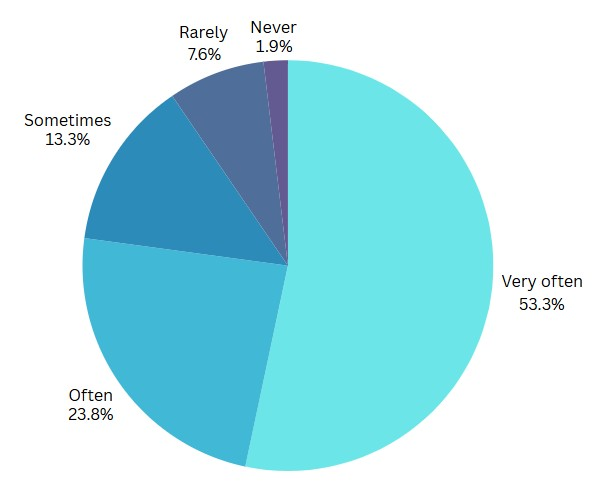
\includegraphics[width=0.6\textwidth]{outings.jpg}
    \caption{Survey: Frequency of Spontaneous Outings}
    \label{fig:spontaneous_outings_new}
\end{figure}

The specific problem we address is the need for a mobile application that provides accurate, real-time table status updates within a restaurant, allowing for efficient management and clear communication to customers. Existing solutions often lack the dynamic, real-time updates essential for addressing the spontaneity of diners and the challenges of peak hours.

\section{Idea Finding}

\subsection{State of the Art}
The restaurant industry in Poland is a dynamic sector, undergoing significant transformations driven by economic shifts, evolving consumer behaviors, and an increasing adoption of technology. Understanding the current landscape of restaurant management and digital solutions within Poland is crucial to positioning the Table Hub Mobile application effectively, by identifying existing gaps and unmet needs in the market.

\subsubsection{Restaurant Industry in Poland}
The Polish foodservice market has experienced substantial quantitative and qualitative changes since the economic transformation of 1989, progressively resembling Western markets \parencite{kowalczuk2015eating}. While its growth rate has stalled in recent years, robust demand, coupled with the rapid development of tourism and business infrastructure, continues to foster expansion \parencite{kowalczuk2015eating}. The market has been largely privatized, with private entities constituting 98\% of outlets in 2013, fostering greater choice and more efficient management \parencite{kowalczuk2015eating}. Historically, simpler catering forms like bars and food stands predominated, but restaurants have recently seen the most significant growth, though bars and food stands still command the largest market share \parencite{kowalczuk2015eating}.

Consumer behavior in Poland indicates that approximately 50\% of Poles utilize catering services, with an average expenditure of 26.2 PLN per month on eating out in 2013 \parencite{kowalczuk2015eating}. However, this expenditure share is considerably lower than the EU average, suggesting a lesser propensity for Poles to dine out frequently \parencite{kowalczuk2015eating}. Spontaneity plays a significant role, with over 74\% of respondents in one survey indicating their outings are spontaneous rather than pre-planned \parencite{kowalczuk2015eating}. This often leads to difficulties, as about 74\% report problems finding a free table during peak hours, particularly on busy days like Fridays and Saturdays \parencite{kowalczuk2015eating}. Key motivations for eating out include taste, reasonable prices, convenience, and time-saving, while financial constraints and the perception of home-cooked meals being healthier are primary barriers \parencite{kowalczuk2015eating}. For tourists in cities like Gdańsk, the taste of meals and appropriate pricing are key incentives for choosing dining options \parencite{pilis2022food}. Individual tourists in Gdańsk tend to favor fast-food, confectioneries, and ice cream parlors over full-service restaurants with waiter service \parencite{pilis2022food}.

Challenges within the Polish foodservice market include a shortage of financial resources for small and medium-sized enterprises, resulting in lower equipment standards and technological advancement \parencite{kowalczuk2015eating}. There is also a perceived scarcity of highly qualified staff and managerial expertise in organization, management, and marketing \parencite{kowalczuk2015eating}. These factors contribute to the persistence of manual, inefficient systems, particularly concerning table management.

\subsubsection{Current Restaurant Management and Reservation Systems in Poland}
The traditional methods of tracking restaurant table availability often rely on manual observation or rudimentary systems, leading to significant inefficiencies, inaccurate information, and potential revenue loss due to mismanaged seating. Customers frequently face uncertainty regarding table availability, and staff can be overwhelmed during peak hours trying to coordinate seating. This problem scales with the size and popularity of the restaurant, as well as the complexity of its layout with multiple sections.

While existing solutions for restaurant management commonly include reservation systems or Point of Sale (POS) integrations , a critical limitation is their typical inability to offer a dynamic, real-time visual representation of table occupancy or an intuitive way for staff to update statuses on the fly. Many solutions track bookings but lack the immediate visual feedback and dynamic adaptability crucial for addressing the spontaneity of diners and the challenges of peak hours. This means that even with a system in place, inefficiencies and customer frustration persist.

Notable examples of systems used or relevant in the Polish market where direct external information (e.g., live website links) is accessible for verification include:
\begin{itemize}
    \item \textbf{GoPOS:} A Polish system providing sales functionalities, mobile waiter solutions, and online ordering. While offering business control and live reporting, it focuses more on transaction processing and less on dynamic, real-time visual table management for staff and direct customer visibility beyond booking \parencite{gopos}.
    \item \textbf{SpotOn:} Offers POS solutions and builds apps for restaurant owners, notably utilizing Kotlin and Jetpack components for app development. Its alignment with modern Android development for the restaurant sector is highly relevant to Table Hub's approach \parencite{spoton}.
    \item \textbf{OpenTable:} A global reservation system active in Poland, it allows customers to book tables online. However, it acts primarily as an intermediary for reservations, and does not provide an interactive, real-time map for general public viewing of instant table availability or for immediate staff updates outside of a formal reservation process \parencite{opentable}.
    \item \textbf{Zjedz.my:} A Polish mobile application for online table booking. Similar to OpenTable, its main utility is for pre-booking, rather than offering real-time, spontaneous table availability checks via a visual interface for immediate seating \parencite{zjedzmy}.
\end{itemize}

Research indicates that restaurants adopting reservation policies generally observe higher spending from customers who book in advance compared to walk-ins, suggesting a financial incentive for implementing efficient systems \parencite{gregorash2016restaurant}. However, manual or rudimentary digital systems often fail to fully capitalize on this potential, leading to lost revenue from mismanaged walk-ins and frustrating peak-hour scenarios. The explicit need for accessible, real-time information to enhance the dining experience and reduce frustration is a significant, currently unmet need.

Capacity management is a critical operational concern in hospitality, impacting customer experience, employee satisfaction, and profitability \parencite{pullman2010capacity}. Short-term capacity decisions involve daily efforts to align capacity with demand, often through flexible seating arrangements and effective queue management \parencite{pullman2010capacity}. Optimizing the table mix, by aligning table configurations with anticipated party sizes, can significantly increase seat occupancy and thus serve more customers without necessitating physical expansion \parencite{kim2020small}. The ability to dynamically manage these elements in real-time, which is often lacking in current solutions, directly impacts a restaurant's ability to maximize revenue and customer satisfaction.

\subsubsection{Digital Transformation in Hospitality and Mobile Application Development}
The hospitality industry is experiencing a profound digital transformation, propelled by advancements in digital technologies (DTs) such as mobile, cloud computing, Internet of Things (IoT), and Artificial Intelligence (AI) \parencite{busulwa2022digital}. This transformation necessitates that hospitality organizations reassess and redesign their operations to achieve greater efficiency, enhance customer experience, improve scalability, and boost strategic agility \parencite{busulwa2022digital}. Correspondingly, hospitality managers require new or enhanced competencies to effectively lead and manage these changes \parencite{busulwa2022digital}.

Mobile applications are pivotal in this digital shift, offering a direct channel to address real-time needs. For instance, the Table Hub Mobile application leverages Kotlin and Jetpack Compose for its user interface. The adoption of Jetpack Compose represents a modern Android development practice that facilitates rapid UI development and a high-quality user experience.

Real-time communication, particularly via WebSockets, is crucial for instantaneous updates and data consistency across all connected clients. This is vital for dynamic table status updates and efficient management. The Table Hub application employs WebSockets for this purpose, managing connections, subscribing to updates, and sending table status changes. This approach offers a significant advantage over older solutions that often lack the dynamic, real-time updates necessary to effectively address the spontaneity of diners and the challenges presented during peak hours. The need for a mobile application that provides accurate, real-time table status updates, allowing for efficient management and clear communication to customers, remains a key problem to be addressed.

\subsection{Innovative Ideas}
We developed the following innovative ideas to address the stated problem, adding new value to better address the stated problem, possibly leading to more effective solutions:
\begin{itemize}
    \item \textbf{Interactive Floor Plan:} A visual, interactive layout of the restaurant with clickable tables to quickly change their status.
    \item \textbf{Real-time WebSocket Communication:} Utilizing WebSockets for instant updates of table statuses across all connected clients, ensuring data consistency.
    \item \textbf{Location-Based Restaurant Discovery:} Enabling users to find nearby restaurants and view their table availability.
    \item \textbf{Filter Options:} Allowing users to filter restaurants based on various criteria like cuisine, rating, and minimum available seats.
    \item \textbf{Intuitive UI with Jetpack Compose:} Building the interface entirely with Jetpack Compose for a modern, reactive, and consistent user experience.
\end{itemize}

\subsection{Main Idea Selection and Justification}
Our team decided to focus on creating a mobile application with an interactive floor plan and real-time WebSocket communication as the core functionalities. We chose this approach because it directly tackles the real-time accuracy and user experience issues we identified. An interactive floor plan provides an immediate visual understanding of the restaurant's state, while WebSockets ensure that this visual representation is always up-to-date for all users. Our user research further indicated a strong potential for a user-driven solution, with \textbf{over 74\% of respondents (30.1\% 'Yes' and 44.7\% 'Maybe') expressing willingness to share real-time information about available places, especially when incentivized by discounts, money, or gamification.} Our use of Jetpack Compose facilitates rapid UI development and a high-quality user interface.

\begin{figure}[H]
    \centering
    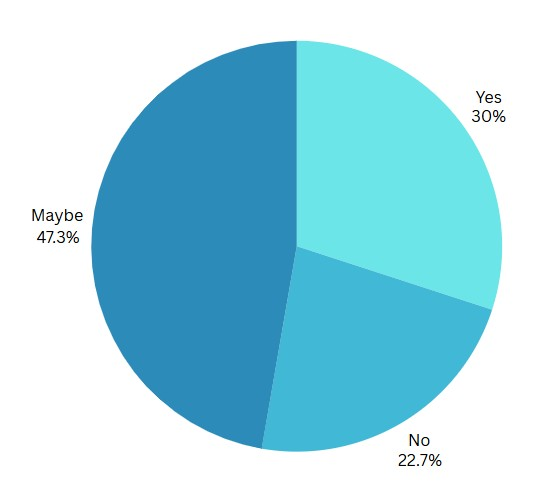
\includegraphics[width=0.6\textwidth]{willingness_to_share.jpg}
    \caption{Survey: Willingness to Share Real-time Information}
    \label{fig:willingness_to_share_new}
\end{figure}

\begin{figure}[H]
    \centering
    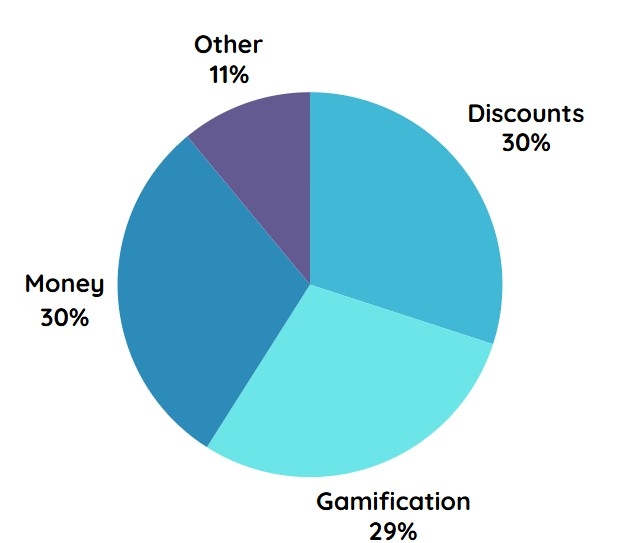
\includegraphics[width=0.6\textwidth]{incentives.jpg}
    \caption{Survey: Incentives for Sharing Information}
    \label{fig:sharing_incentives_new}
\end{figure}

\section{Solution Implementation}
The Table Hub Mobile application is an Android application developed in Kotlin, leveraging modern Android development practices, including Jetpack Compose for UI and Hilt for dependency injection. The application communicates with a backend service via WebSockets to manage restaurant and table data in real-time.

\subsection{Technical Details}
The application's architecture follows a MVVM (Model-View-ViewModel) pattern, integrated with a repository pattern for data management and services for business logic and network communication.

\subsubsection{Core Components}
\begin{itemize}
    \item \textbf{Activities:} \texttt{MainActivity} serves as the single activity host for the application's fragments.

    \item \textbf{Fragments:}
    \begin{itemize}[leftmargin=2em]
        \item \texttt{LogInFragment}: Handles user authentication.
        \item \texttt{MainViewFragment}: Displays the main map view with restaurants and allows navigation to other features.
        \item \texttt{ReportViewFragment}: Shows a list of restaurants for reporting purposes.
        \item \texttt{RestaurantLayoutFragment}: Displays the interactive layout of a selected restaurant's tables.
        \item \texttt{SettingsFragment}: Provides settings options.
    \end{itemize}

    \item \textbf{ViewModels:}
    \begin{itemize}[leftmargin=2em]
        \item \texttt{MainViewViewModel}: Manages UI-related data for the main map view, including restaurants and user location, and handles fetching user location.
        \item \texttt{ReportViewViewModel}: ViewModel for the report view.
    \end{itemize}

    \item \textbf{Services:}
    \begin{itemize}[leftmargin=2em]
        \item \texttt{TablesService} (interface) and \texttt{TablesServiceImplementation}: Define and implement the core logic for table status updates, interacting with the \texttt{WebSocketService}.
        \item \texttt{WebSocketService}: Manages WebSocket connections and communication with the backend server for real-time data exchange. It handles connecting, subscribing to updates, and sending table status changes.
        \item \texttt{MockTableService}: A mock implementation of \texttt{TablesService} for testing and development purposes.
    \end{itemize}

    \item \textbf{Repositories:}
    \begin{itemize}[leftmargin=2em]
        \item \texttt{IRestaurantsRepository} (interface) and \texttt{RestaurantsRepositoryImpl}: Abstract and implement the data layer for managing restaurant information, including processing initial data and table status changes.
    \end{itemize}

    \item \textbf{Models:} Data classes representing core entities like \texttt{Location}, \texttt{Position}, \texttt{Restaurant}, \texttt{Section}, \texttt{Table}, and \texttt{TableStatus}. WebSocket-specific models (e.g., \texttt{WebSocketMessage}, \texttt{MessageType},\\ \texttt{TableUpdateRequest}) are also defined.

    \item \textbf{Dependency Injection:} Hilt is used for dependency injection, making the application components easily testable and managing their lifecycle. Modules like \texttt{ClientModule}, \\ \texttt{MessageProcessorModule}, and \texttt{RepositoryModule} provide instances of WebSocket clients, message processors, and repositories.

    \item \textbf{UI (Jetpack Compose):} The user interface is built declaratively using Jetpack Compose. Examples include \texttt{MainLoginView}, \texttt{MainMapView}, \texttt{RestaurantLayoutMainView}, and various reusable composables for buttons, text fields, and pop-ups.
\end{itemize}

\subsubsection{Key Features and Implementations}
\begin{itemize}
    \item \textbf{Location Services:} The \texttt{MainViewViewModel} requests and fetches the user's last known location using \texttt{LocationServices.getFusedLocationProviderClient}. Necessary permissions (\texttt{ACCESS\_FINE\_LOCATION}, \texttt{ACCESS\_COARSE\_LOCATION}) are declared in \texttt{AndroidManifest.xml} and handled at runtime.

    \item \textbf{Map Integration:} The \texttt{MapboxMapWrapper} composable integrates Mapbox for displaying restaurants on a map. Custom markers are created to show the number of available tables.

    \item \textbf{Real-time Communication:} The \texttt{WebSocketService} establishes and manages a STOMP (Simple Text Oriented Messaging Protocol) WebSocket connection. It subscribes to \texttt{/topic/restaurant/status} for initial status and \texttt{/user/queue/updateTableStatus} for table updates, and sends updates to \texttt{/app/updateTableStatus}. The \texttt{WSMessageRelay} acts as a central hub for WebSocket messages.

    \item \textbf{Data Processing:} The \texttt{WebsocketMessageProcessorImpl} observes the \texttt{WSMessageRelay} and processes incoming WebSocket messages based on their \texttt{MessageType} (e.g., \texttt{QUERY\_RESTAURANTS\_RESPONSE}, \texttt{SUBSCRIBE\_RESTAURANT\_UPDATES\_RESPONSE}, \texttt{TABLE\_STATUS\_CHANGED\_EVENT}), updating the \\ \texttt{RestaurantsRepositoryImpl} accordingly.

    \item \textbf{Table Status Update:} Within \texttt{RestaurantLayoutFragment}, users can select a section and then tap on individual tables to change their status (\texttt{AVAILABLE}, \texttt{OCCUPIED}, \texttt{UNKNOWN}) via an \texttt{AlertDialog}. These updates are then sent to the backend through the \texttt{TablesServiceImplementation}.

    \item \textbf{User Interface Styling:} The app defines its color scheme in \texttt{colors.xml} and \texttt{Color.kt}, and themes in \texttt{themes.xml} and \texttt{Theme.kt}, providing a consistent visual identity. String resources for localization are available in \texttt{strings.xml} and \texttt{strings-pl.xml}.
\end{itemize}

\subsubsection{UML Diagrams}

\begin{figure}[H]
    \centering
    \includegraphics[width=0.8\textwidth]{ui_uml.jpg}
    \caption{UI Component Diagram}
    \label{fig:ui_uml}
\end{figure}

This diagram (Figure \ref{fig:ui_uml}) illustrates the hierarchy and interaction of the main UI components, showing how fragments and activities are structured and how they relate to the overall application flow. It also depicts the connection to external components like \texttt{MainViewComponent} and \texttt{LoginComponent}.

\begin{figure}[H]
    \centering
    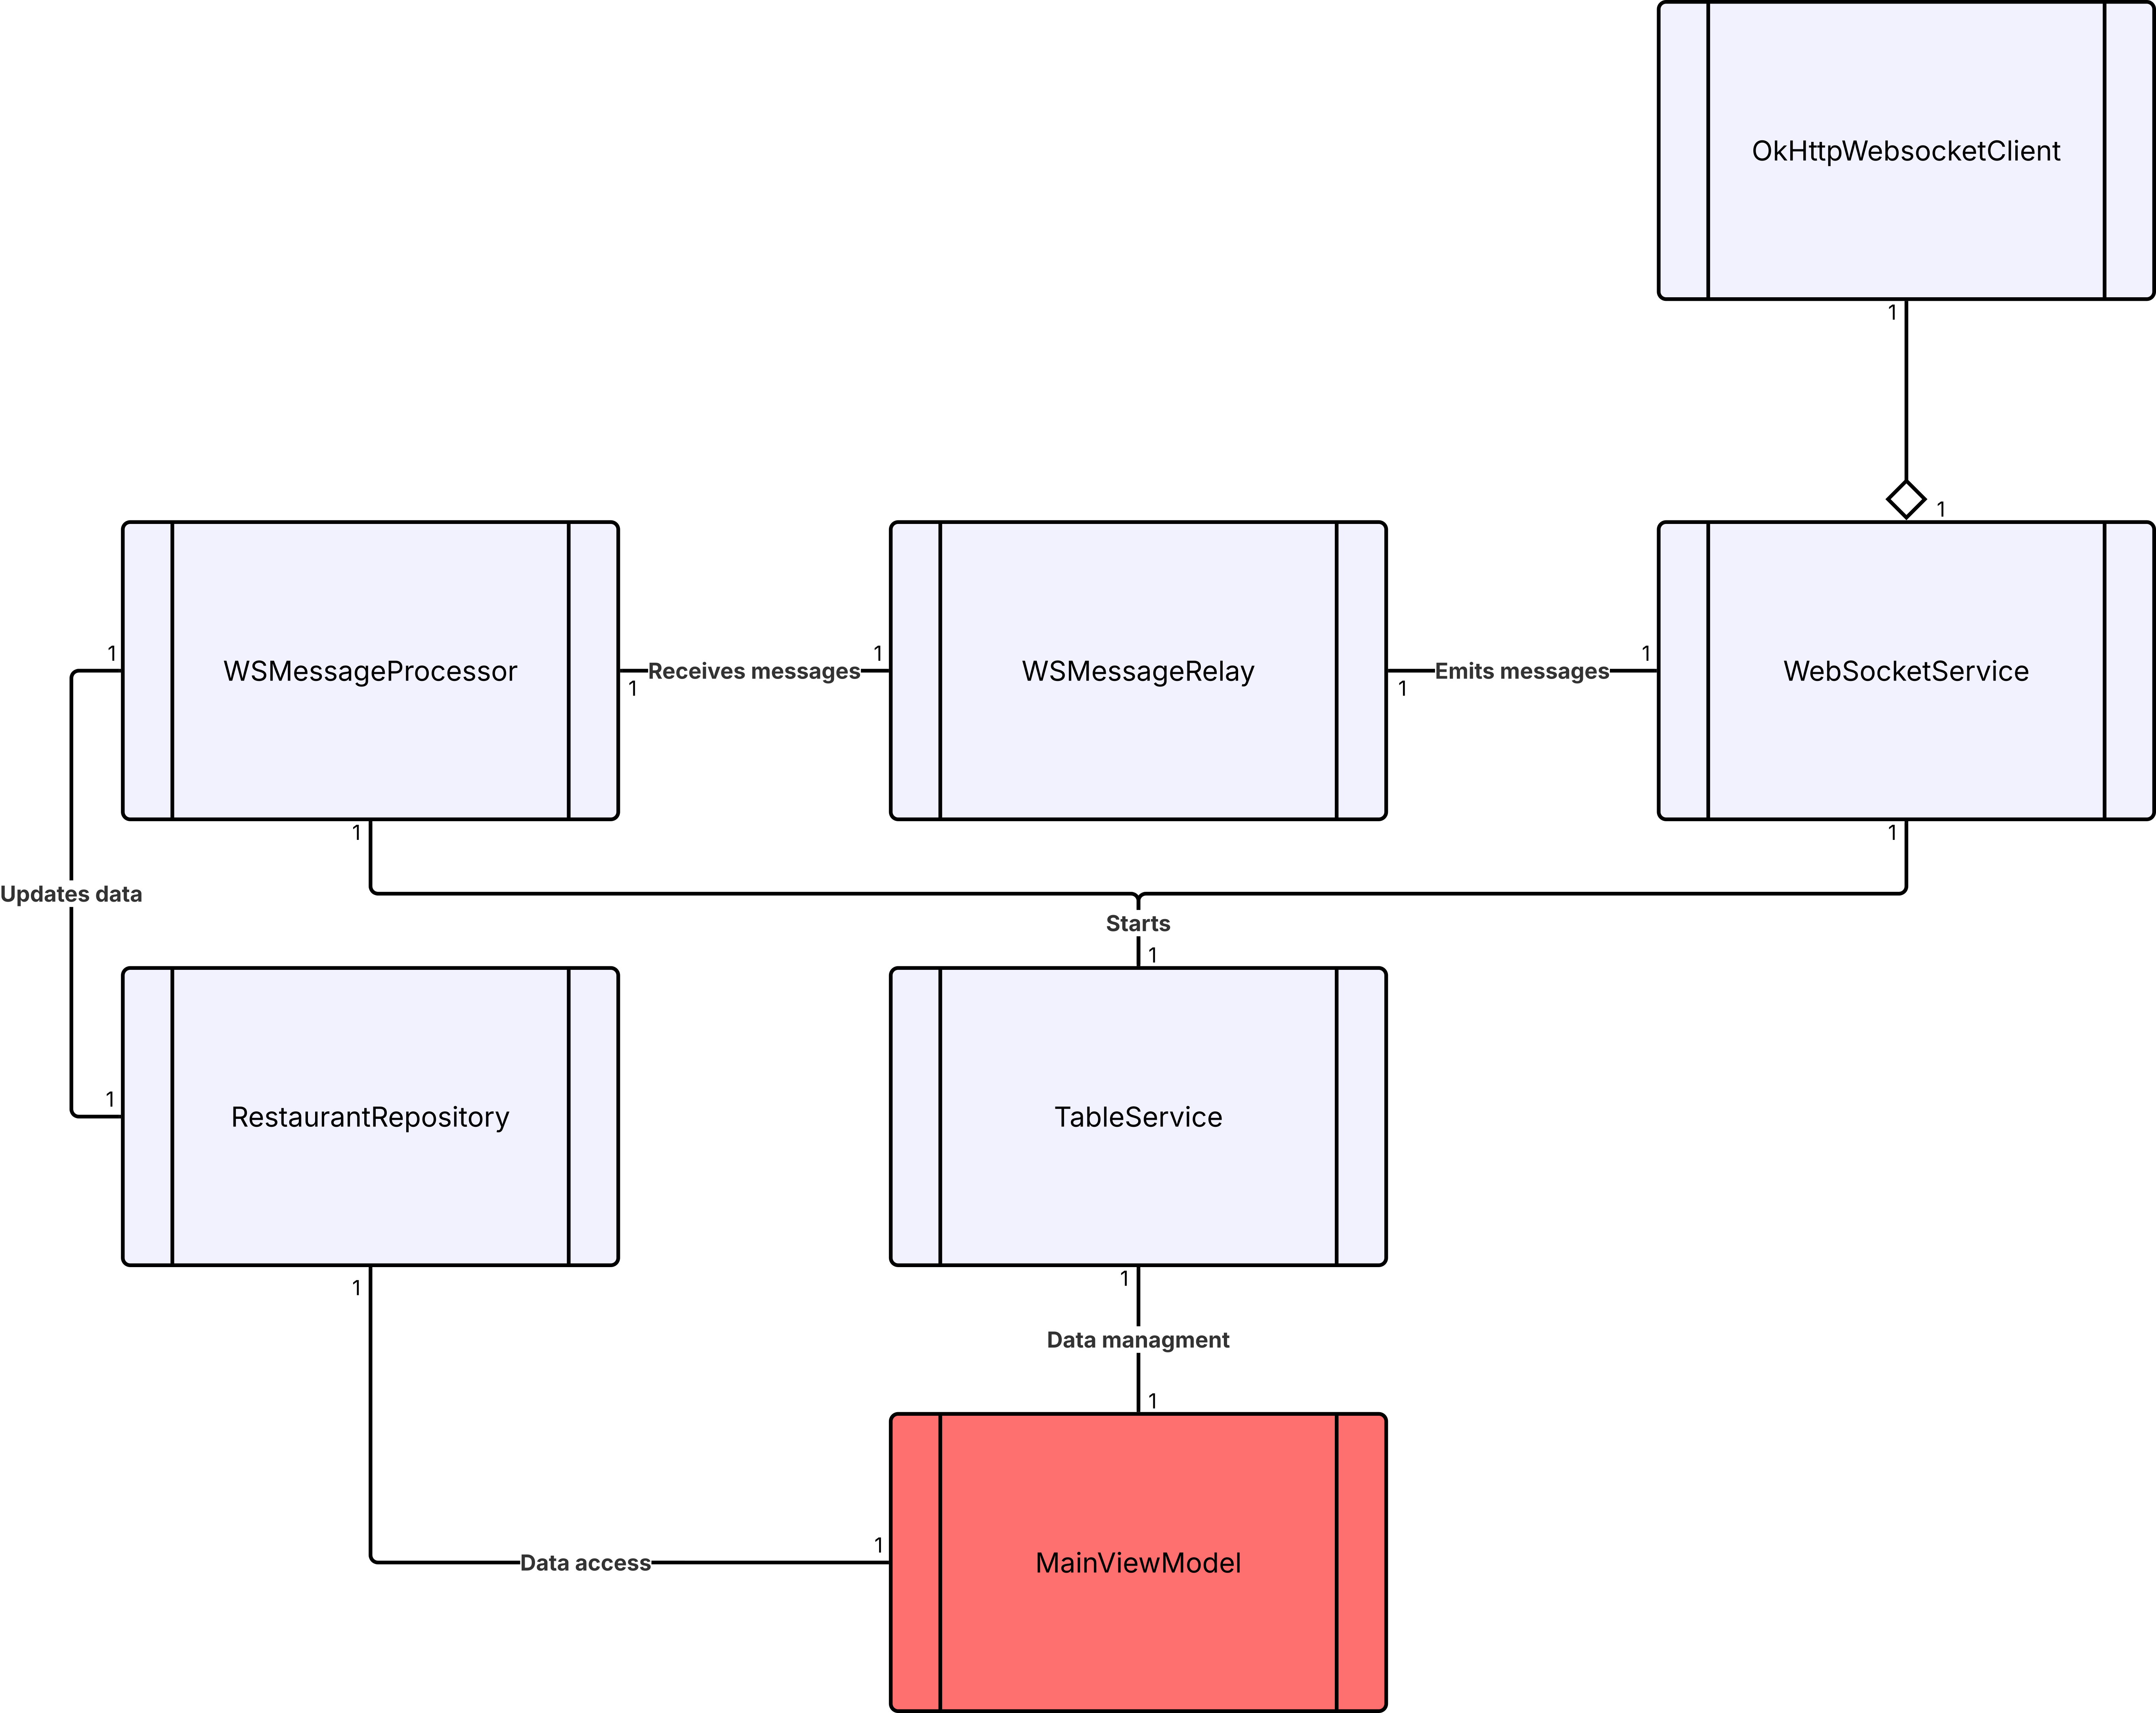
\includegraphics[width=0.8\textwidth]{service_uml.jpg}
    \caption{Service and Repository Interaction Diagram}
    \label{fig:service_uml}
\end{figure}

As seen in Figure \ref{fig:service_uml}, this diagram details the relationships between the WebSocket communication components (\texttt{OkHttpWebsocketClient}, \texttt{WebSocketService}), the message processing logic (\texttt{WSMessageRelay}, \texttt{WSMessageProcessor}), and the data layer (\texttt{RestaurantRepository}). It highlights how the \texttt{MainViewViewModel} accesses data and how \texttt{TablesService} initiates data management.

\begin{figure}[H]
    \centering
    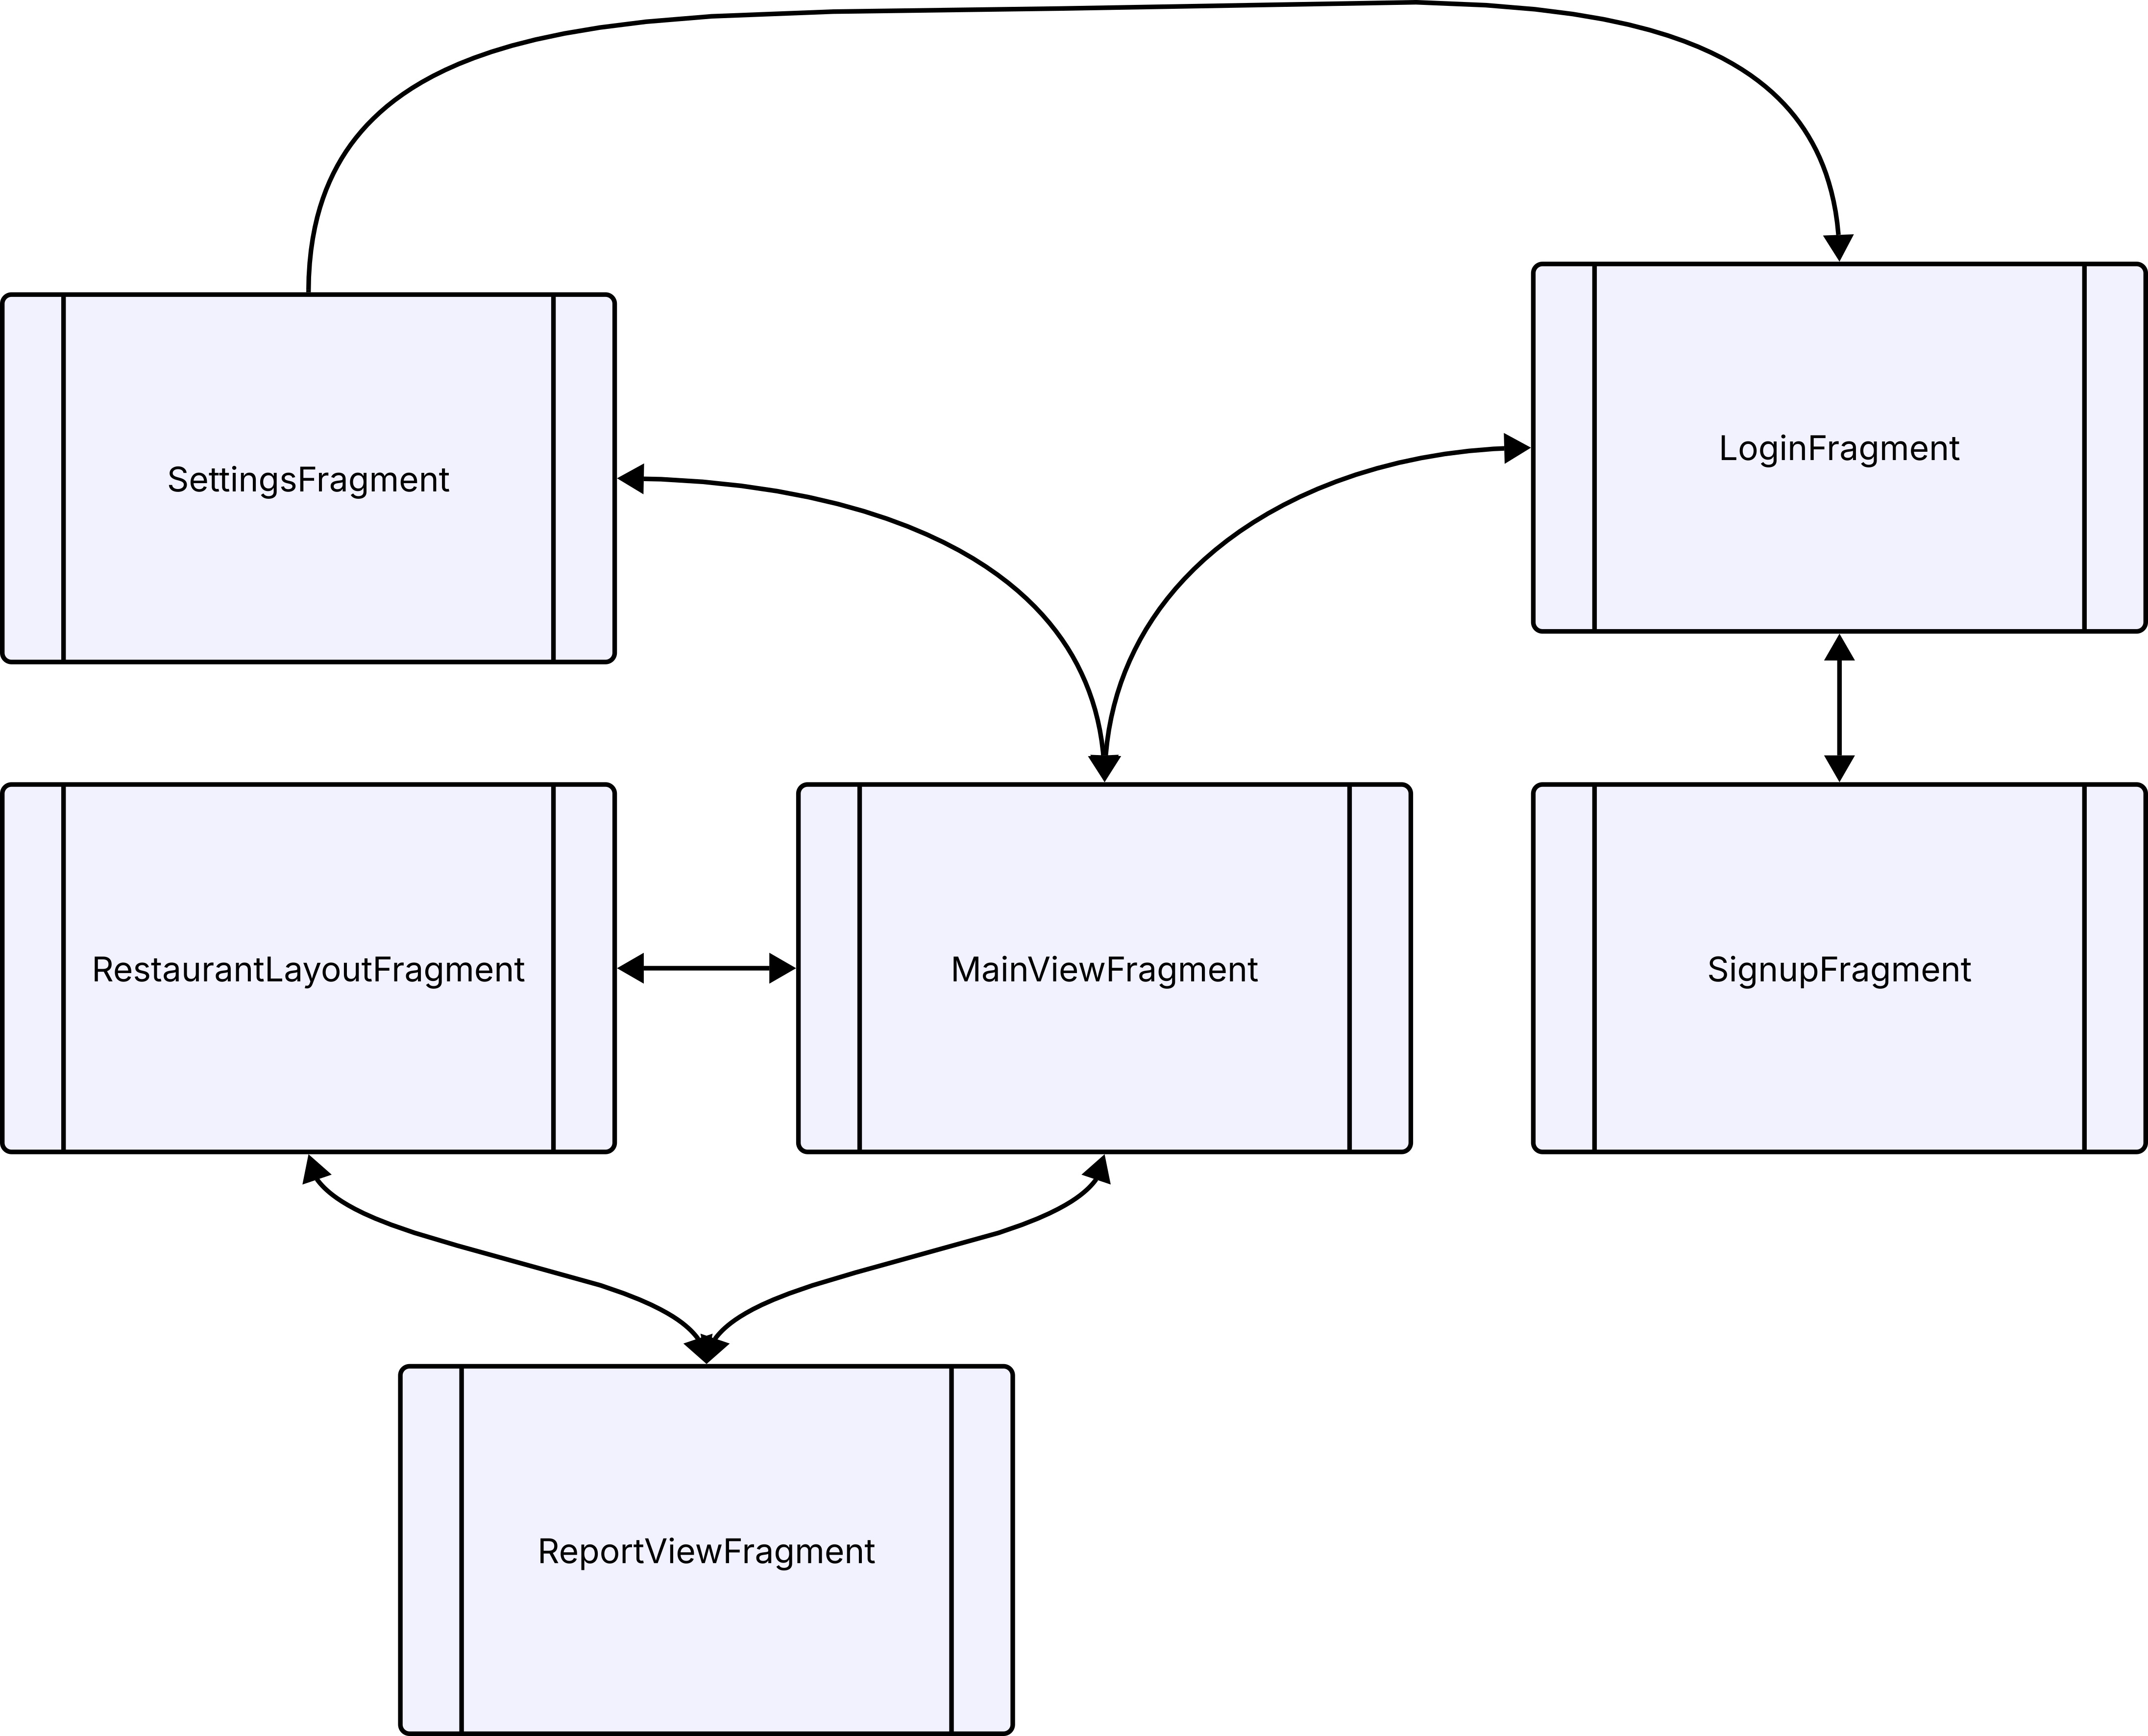
\includegraphics[width=0.8\textwidth]{nav_graph.jpg}
    \caption{Navigation Graph Diagram}
    \label{fig:nav_graph}
\end{figure}

The navigation graph (Figure \ref{fig:nav_graph}) visually represents the flow between different fragments in the application. It shows the possible transitions between \texttt{LogInFragment}, \texttt{SignupFragment}, \texttt{MainViewFragment}, \texttt{SettingsFragment}, \texttt{ReportViewFragment}, and \texttt{RestaurantLayoutFragment}.

\section{Ways of Verification}
The solution's effectiveness can be verified through a combination of unit testing, integration testing, and user acceptance testing.

\begin{itemize}
    \item \textbf{Unit Tests:} We test individual components, especially business logic in ViewModels and data handling in Repositories, in isolation. For example, \texttt{ExampleUnitTest.kt} demonstrates a basic unit test for an addition function.

    \item \textbf{Integration Tests:} We perform testing of the interaction between different layers, such as a ViewModel interacting with a Repository, or the \texttt{TablesServiceImplementation} with the \texttt{WebSocketService}, to ensure proper data flow and communication.

    \textbf{UI Tests (Instrumented Tests):} Using AndroidX Test and Espresso (or Compose testing APIs), we test the UI components and navigation flows on an actual device or emulator. \texttt{ExampleInstrumentedTest.kt} shows a basic instrumented test verifying the app's package name.

    \item \textbf{User Acceptance Testing (UAT):} Real users (restaurant staff and customers) would interact with the application in a live environment to validate its usability, functionality, and ability to solve the problem efficiently. Key metrics would include the time taken to update table statuses, accuracy of reported availability, and overall user satisfaction.
\end{itemize}

\section{Conclusions and Perspectives}
The Table Hub Mobile application offers a robust and intuitive solution for real-time restaurant table management. Its modular architecture, leveraging Kotlin, Jetpack Compose, and Hilt, promotes maintainability and scalability. The integration of WebSockets ensures that table status updates are instant and synchronized across all users.

\subsection{Strengths}
\begin{itemize}
    \item Real-time data synchronization.
    \item User-friendly and interactive UI for table management.
    \item Clear separation of concerns through MVVM and Repository patterns.
    \item Leverages modern Android development tools.
\end{itemize}

\subsection{Weaknesses}
\begin{itemize}
    \item \textbf{Fixed WebSocket URL:} The application currently relies on a hardcoded WebSocket server URL. This limits flexibility and would need to be made configurable for broader deployment.

    \item \textbf{Basic WebSocket Error Handling:} Error handling for WebSocket communication could be improved. Implementing retry mechanisms or more robust user notifications for connection issues would enhance reliability.
\end{itemize}

\subsection{Potential Follow-up}
\begin{itemize}
    \item \textbf{Backend Integration:} Develop the full backend service to complement the mobile application, ensuring secure and scalable data storage.

    \item \textbf{User Authentication and Profiles:} Implement a complete user authentication system with different roles (e.g., staff, customer) and personalized profiles.

    \item \textbf{Reservation System Integration:} Extend functionality to include table reservation capabilities directly within the app.

    \item \textbf{Notifications:} Implement push notifications for significant events, such as a requested table becoming available.

    \textbf{Admin Panel:} Create a web-based admin panel for restaurant owners to manage their layouts, sections, and tables.

    \item \textbf{Improved Location Accuracy:} Integrate more advanced location services or manual location input for better accuracy.
\end{itemize}

\appendix
\section*{Appendix}

\subsection*{App Views}

\begin{figure}[H]
    \centering
    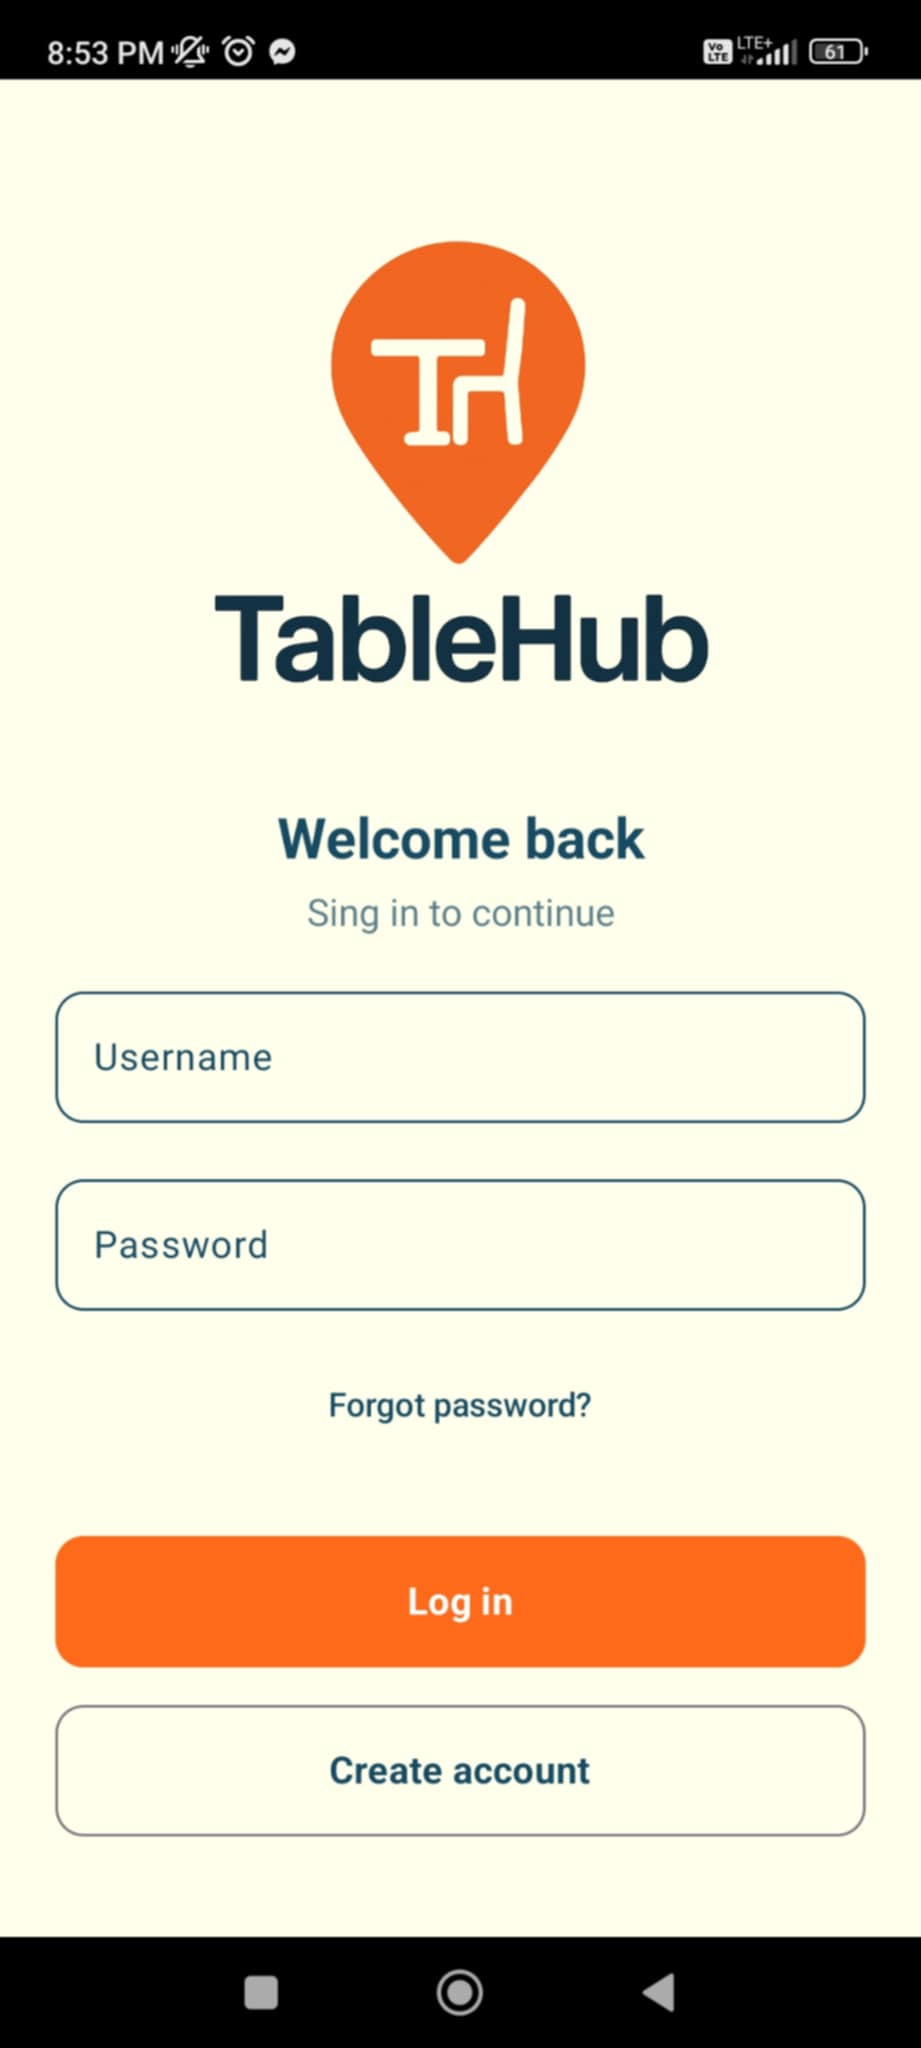
\includegraphics[width=0.5\textwidth]{log_in_screen.jpg}
    \caption{Login Screen}
    \label{fig:login_screen}
\end{figure}

This view provides user authentication, allowing existing users to log in and offering options for new account creation or password recovery.

\begin{figure}[H]
    \centering
    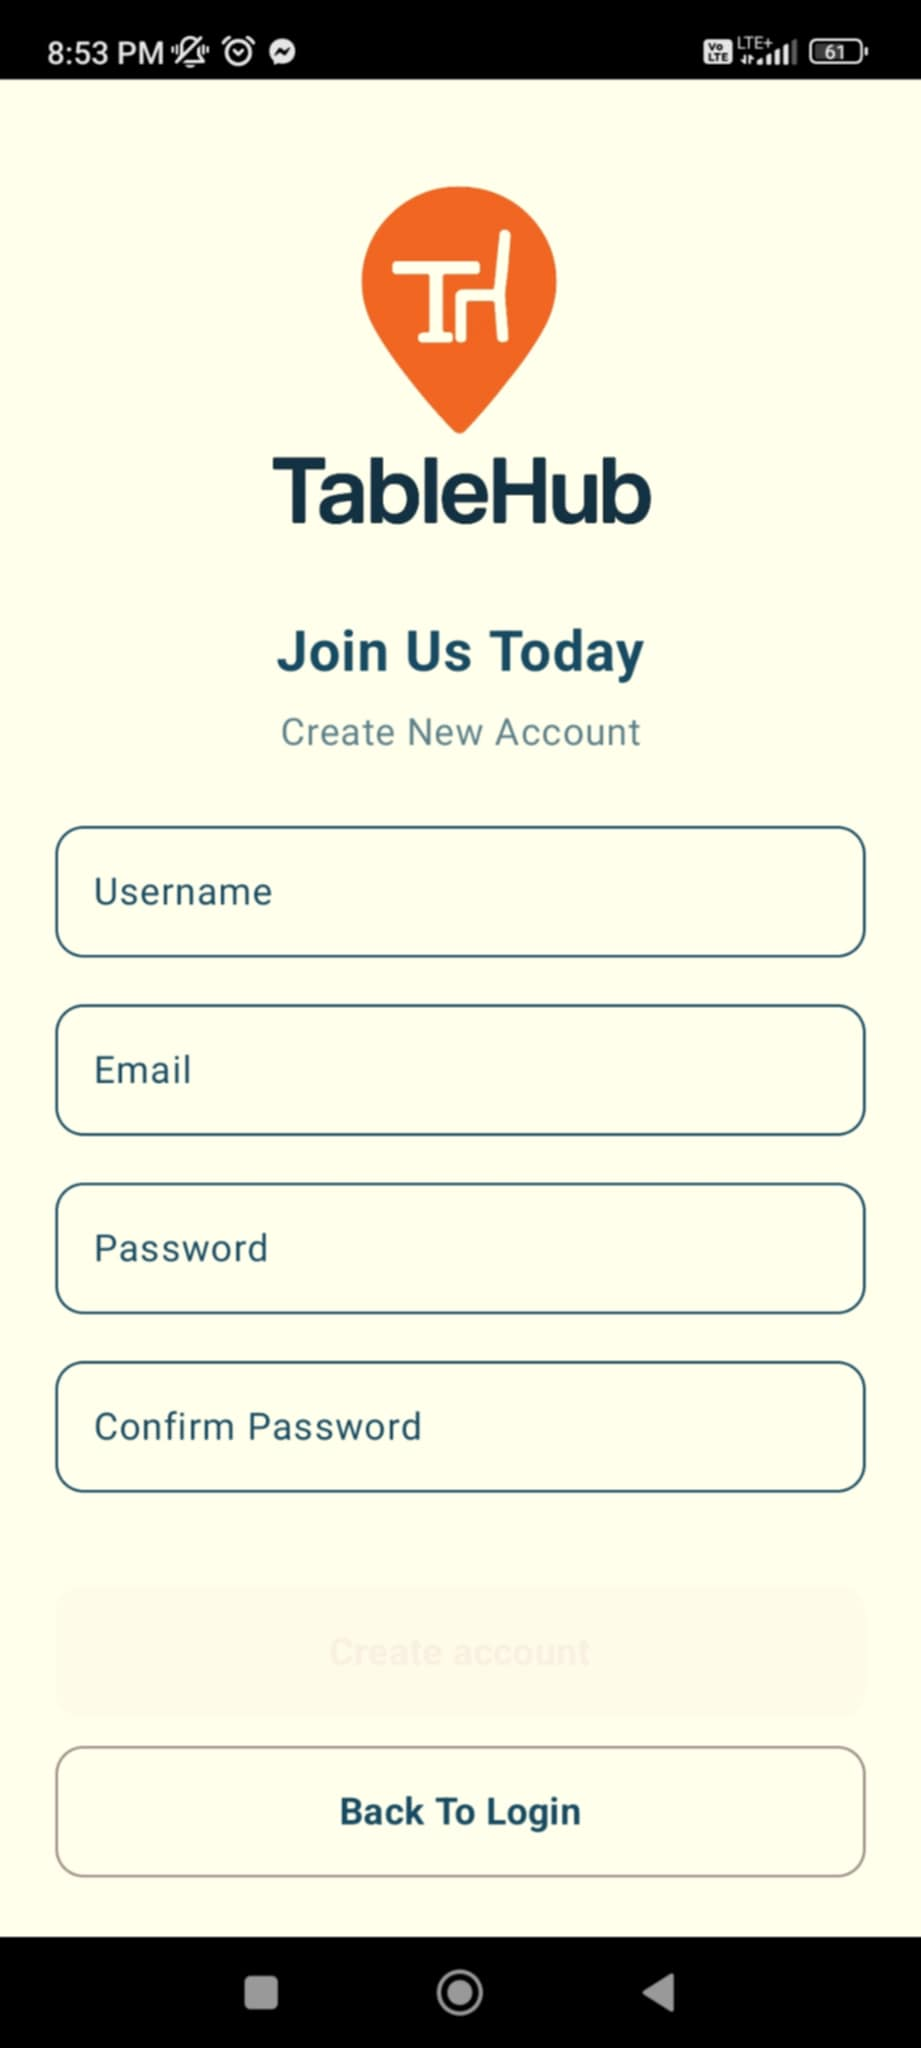
\includegraphics[width=0.5\textwidth]{sign_in_screen.jpg}
    \caption{Sign Up Screen}
    \label{fig:signup_screen}
\end{figure}

This view facilitates new user registration, capturing necessary details for account creation.

\begin{figure}[H]
    \centering
    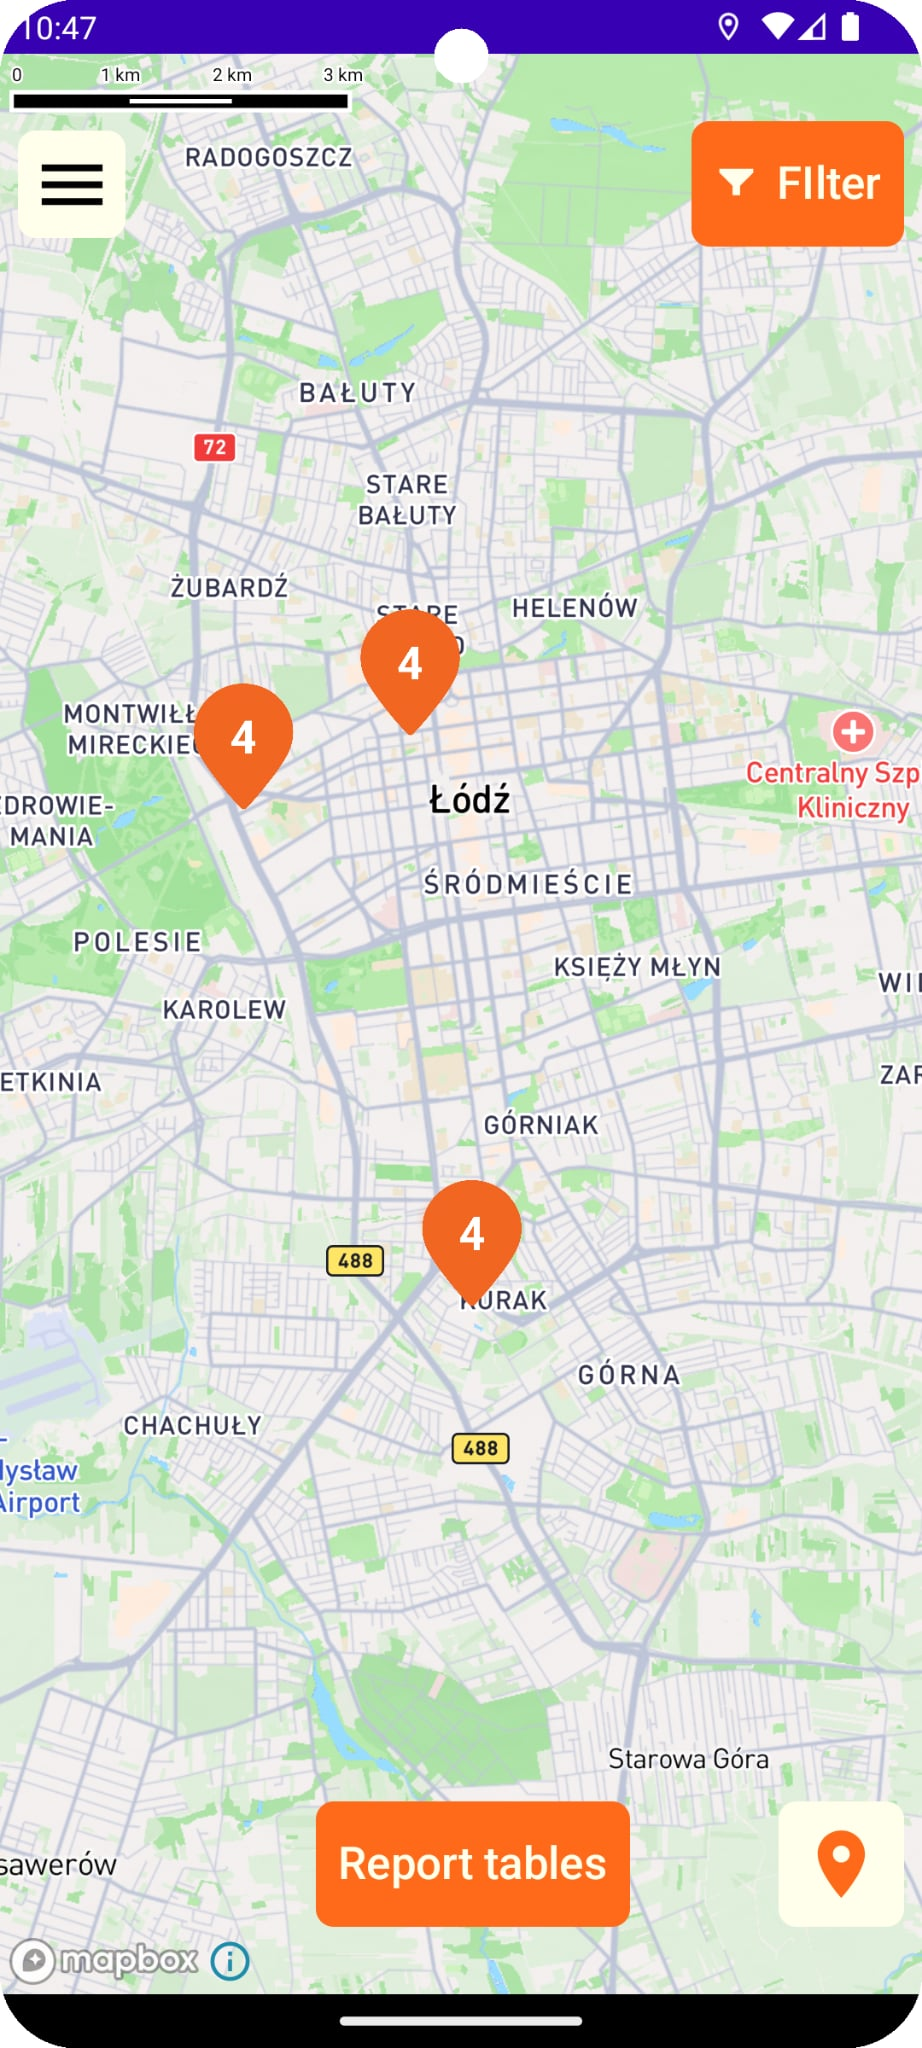
\includegraphics[width=0.5\textwidth]{map_view.jpg}
    \caption{Map View with Restaurants}
    \label{fig:map_view}
\end{figure}

This map-based interface enables users to discover nearby restaurants, with visual markers indicating table availability and access to filtering options.

\begin{figure}[H]
    \centering
    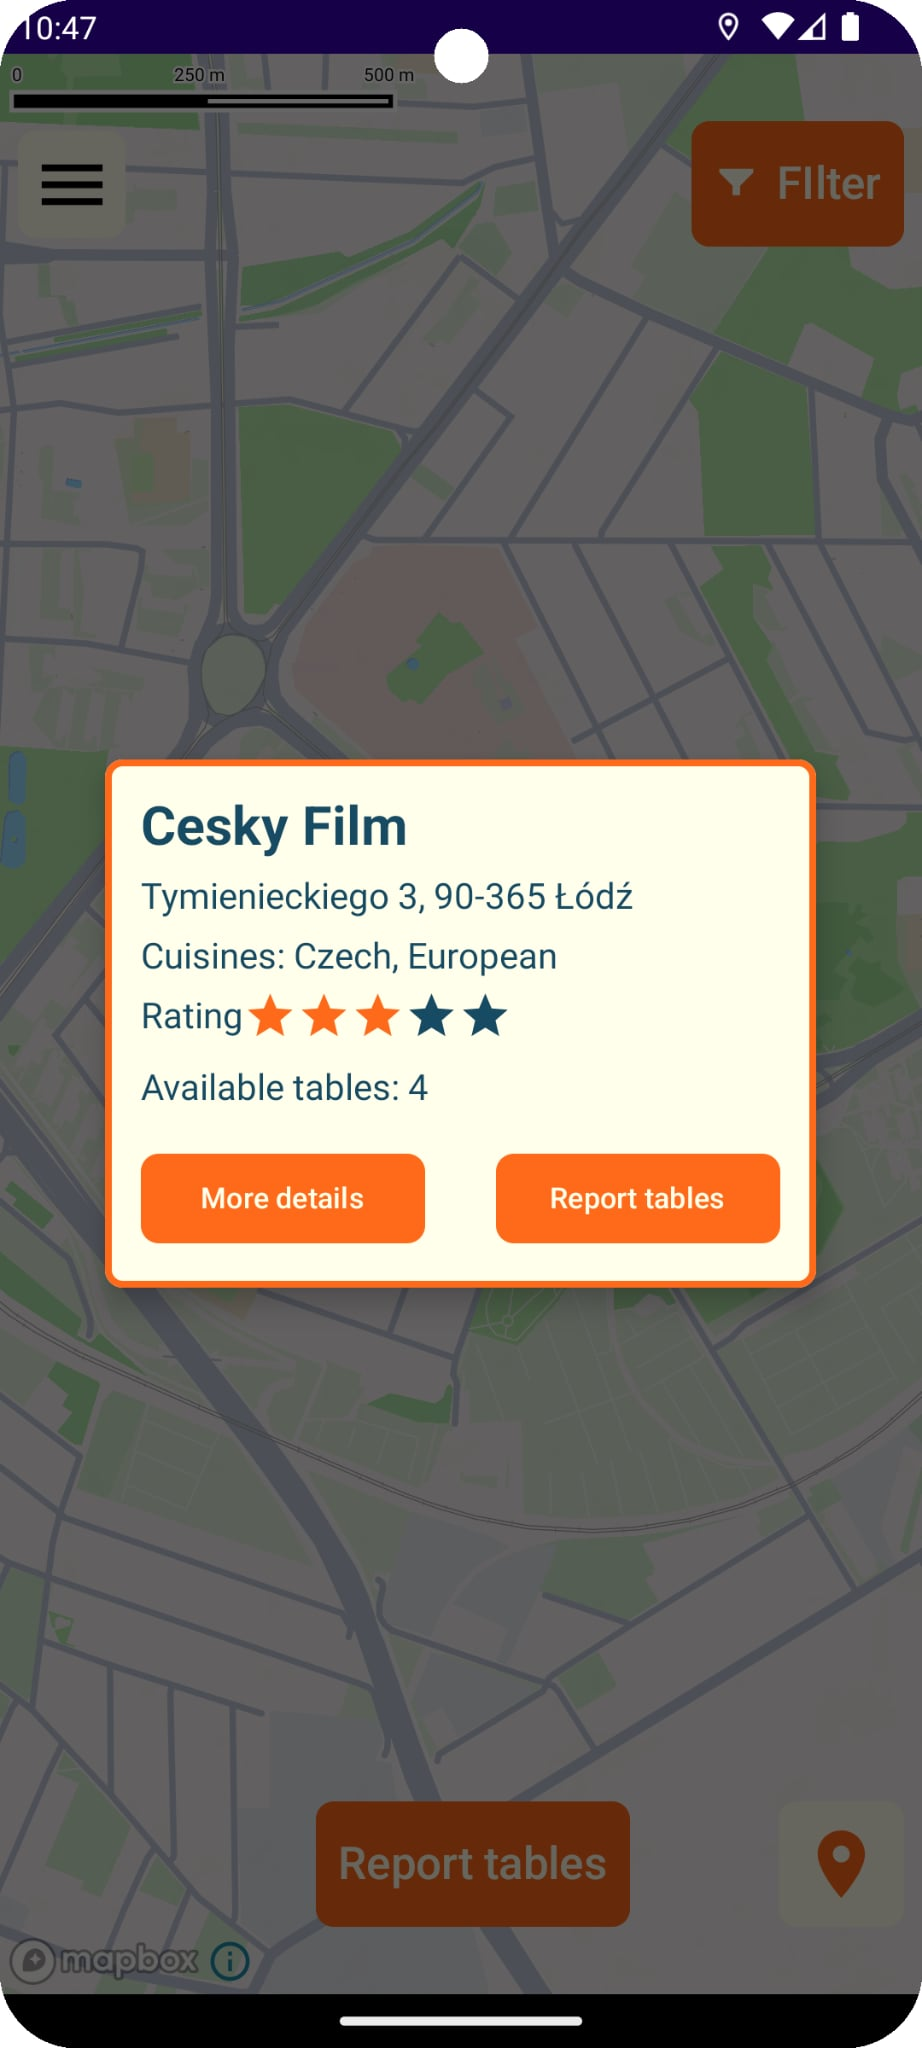
\includegraphics[width=0.5\textwidth]{restaurant_info.jpg}
    \caption{Restaurant Information Pop-up on Map View}
    \label{fig:restaurant_info}
\end{figure}

This pop-up presents concise details for a selected restaurant from the map, including address, cuisine, rating, and available tables, with options for further action.

\begin{figure}[H]
    \centering
    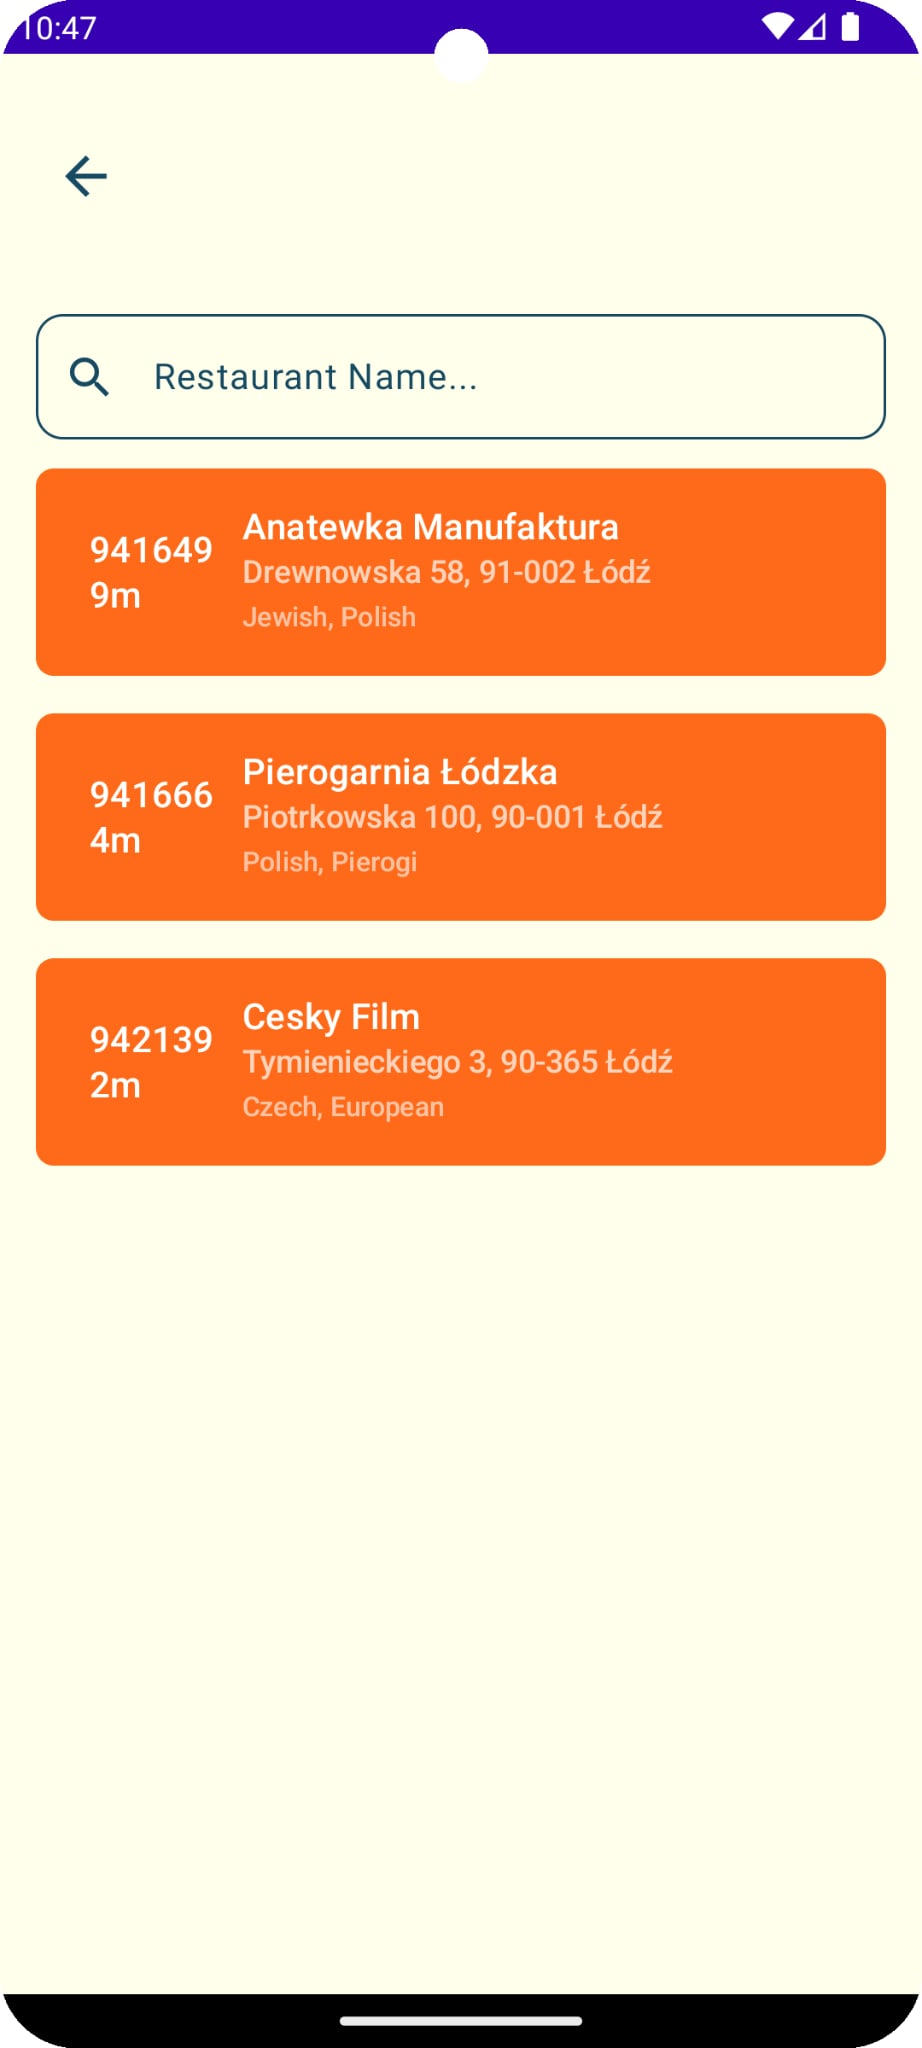
\includegraphics[width=0.5\textwidth]{restaurant_search.jpg}
    \caption{Restaurant Search and List View}
    \label{fig:restaurant_search}
\end{figure}

This interface allows users to search for restaurants by name and browse results in a list format, displaying key information like name, address, distance, and cuisine.

\begin{figure}[H]
    \centering
    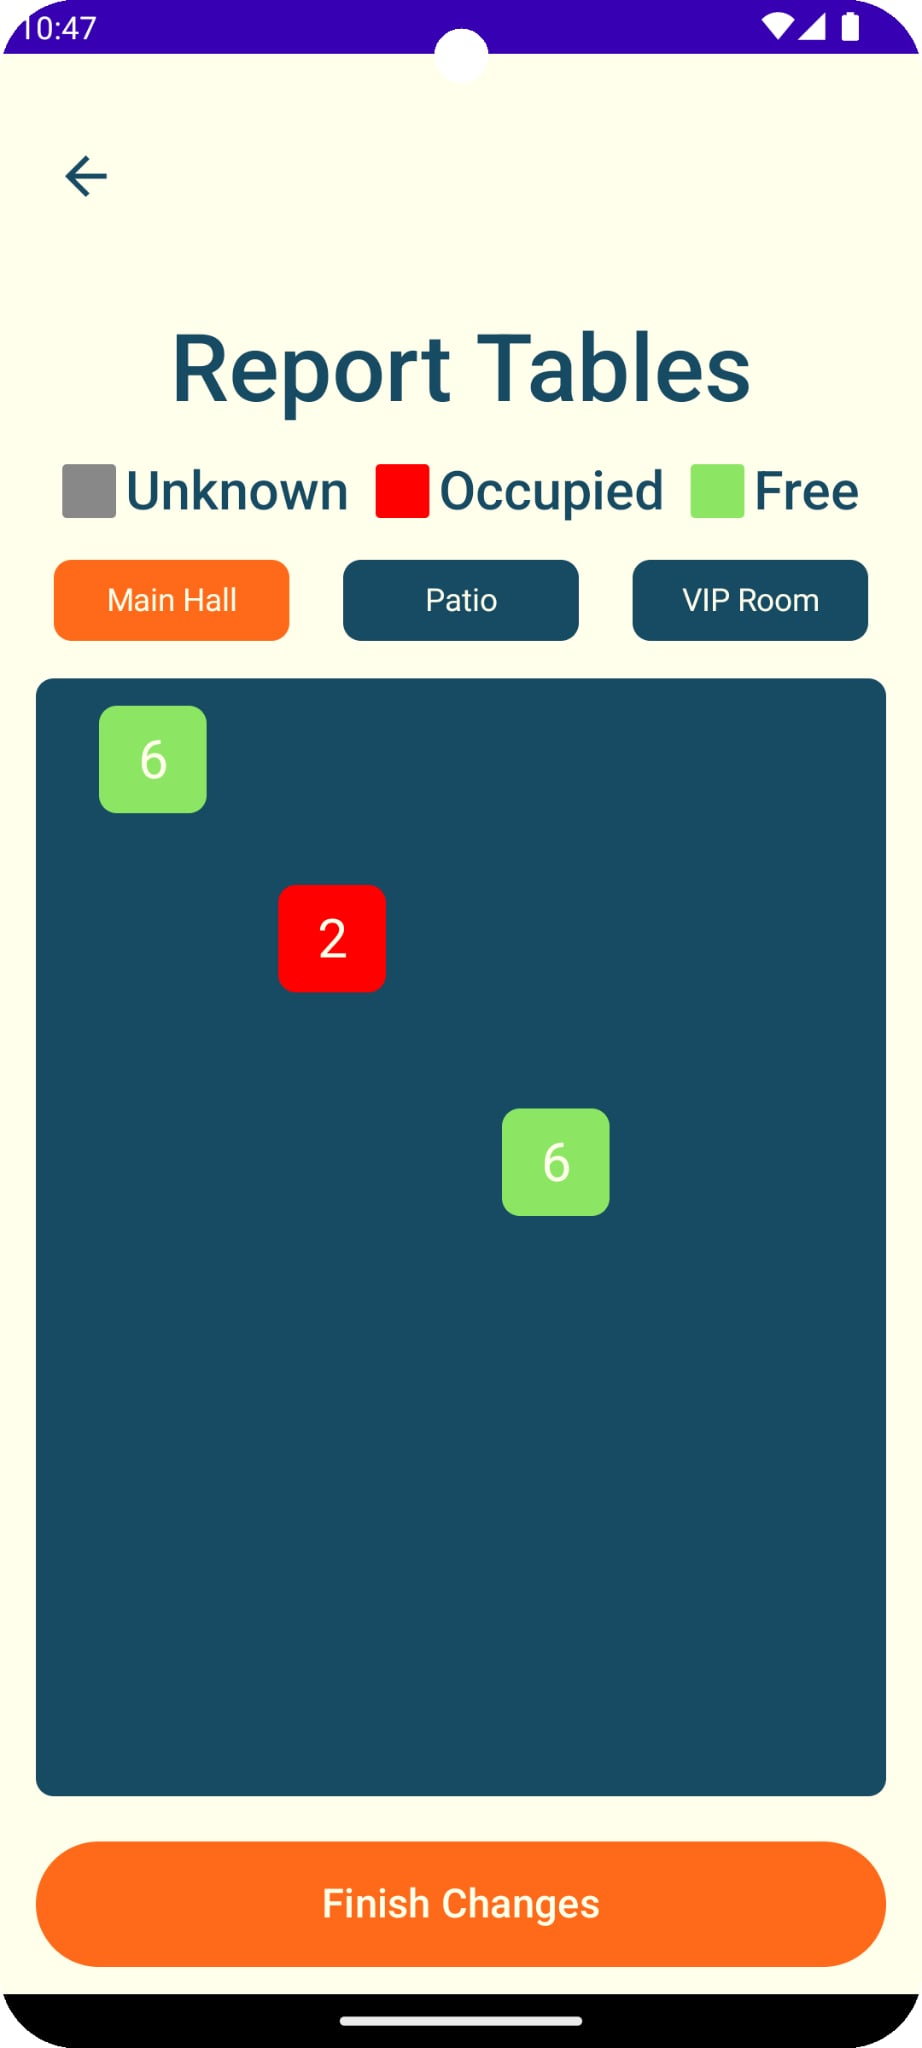
\includegraphics[width=0.5\textwidth]{tables_view.jpg}
    \caption{Interactive Table Layout View}
    \label{fig:tables_view}
\end{figure}

This interactive view presents a visual floor plan of a restaurant section, distinguishing tables by their current status (e.g., free, occupied) and allowing users to initiate status changes.

\begin{figure}[H]
    \centering
    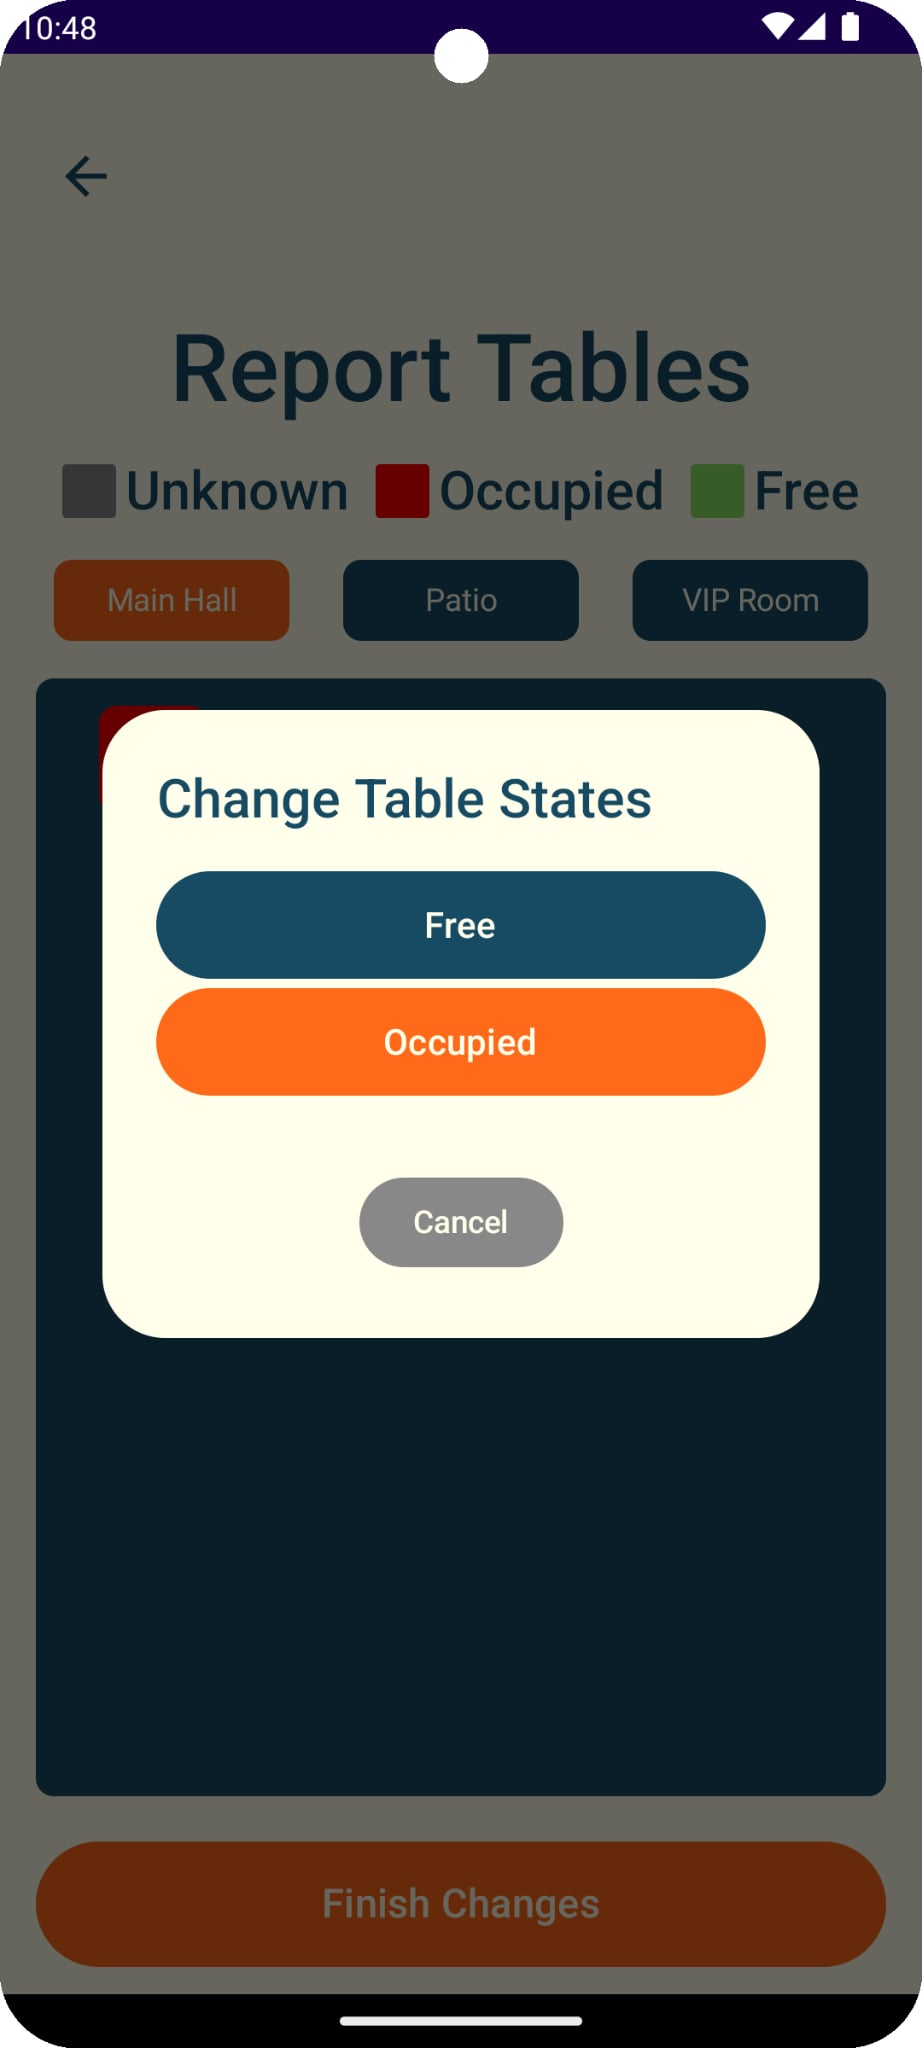
\includegraphics[width=0.5\textwidth]{report_tables.jpg}
    \caption{Change Table States Dialog}
    \label{fig:report_tables_dialog}
\end{figure}

This dialog allows users to update the status of a selected table (e.g., to 'Free' or 'Occupied'), facilitating real-time status reporting.

\subsection*{Code Repository}
\url{https://github.com/Table-Hub-TUL}

\section*{Acknowledgment}
We would like to express our sincere gratitude to our supervisor, \supervisorname{}, for his invaluable guidance and support throughout this project. His expertise and encouragement were instrumental in bringing Table Hub Mobile to fruition.

\clearpage % Ensures the bibliography starts on a new page

\printbibliography 
\end{document}